%%%  default
\documentclass[10pt, compress]{beamer}


\usetheme{mnuigD}
\usepackage{tikz}
\usepackage{booktabs}
%\usepackage{cite}
\bibliographystyle{apalike}
\usepackage[export]{adjustbox}
\usepackage{subfig}
\usepackage[export]{adjustbox}
% \usepackage[scale=2]{ccicons}
\usepackage[normalem]{ulem} % for strikethorugh
%\usemintedstyle{trac}
\usepackage{grffile} %for underscores in file names
\title{The significance of the p-value in 2017}
%\subtitle{{\small (or, smoke and mirros)}}
% \subtitle{NUIG Bioinformatics}
\date{\footnotesize{ Hot Topic: \today}}
\author{
  % \vspace{10mm}
  % \hspace{5mm}
\includegraphics[height=30mm]{./20170202_bss_figs/logo_1_dark}
\\ \\ \\ \\ \large{Nick Waters}}
\institute{
National University of Ireland, Galway\\
James Hutton Institute, Dundee}

%%%%% %%%%% %%%%% %%% %%%%  for pretty headers with pictures
\addtobeamertemplate{frametitle}{}{%
\begin{tikzpicture}[remember picture,overlay]
\node[anchor=north east,yshift=2pt] at (current page.north east) {
\includegraphics[height=0.8cm]{../stock_logos/nuig_rounded.png}  \hspace*{.05cm} 
\includegraphics[height=.794cm, trim= 0cm 0.0cm 0.0cm 0cm]{../stock_logos/jhi_rounded.png}};
\end{tikzpicture}}
%%%%%%%%
\usepackage{xcolor}
\newcommand\ytl[2]{
\parbox[b]{8em}{\hfill{\color{cyan}\bfseries\sffamily #1}~$\cdots\cdots$~}\makebox[0pt][c]{$\bullet$}\vrule\quad \parbox[c]{4.5cm}{\vspace{7pt}\color{red!40!black!30}\raggedright\sffamily #2.\\[7pt]}\\[-3pt]}


%%%%%%%%%%%%%%%%%%%%%%%%%%%%%%%%%%%%%%

\begin{document}
\maketitle

%\maketitle
\setbeamertemplate{itemize items}[square]

\section{The problem with statistics in research}

\begin{frame}[fragile]
  \frametitle{}
  \begin{itemize}
  \item Lack of reproducibility across fields
  \item Irresponsible handling of results
    \begin{itemize}
    \item p-hacking
    \item ignoring multiple comparisons
      \end{itemize}
  \item Publication bias
  \item Lack of power
  \end{itemize}
\end{frame}


\begin{frame}{2017: a year of p-value controversy }
\begin{table}
%\caption{Timeline of something.}
\centering
\begin{minipage}[t]{.7\linewidth}
\color{gray}
\rule{\linewidth}{1pt}
\ytl{July22}{Redefining Statistical Significance [Benjamin et al]}
\ytl{July24}{Eliminate The P-Value (and Bayes Factor) Altogether [Briggs]}
\ytl{Sept21}{Abandon Statistical significance [McShane, et al] }
\bigskip
\rule{\linewidth}{1pt}%
\end{minipage}%
\end{table}
\end{frame}

\section{A refresher}
\begin{frame}[fragile]
  \frametitle{Reminder: NHST}
  NHST: Null hypothesis significance testing
  A p-value is the odds of seeing your result by accident if there is not effect.
  \begin{itemize}
  \item p < 0.05 : the null hypothesis might be able to be rejected
  \item p > 0.05 : the null hypothesis doesn't deserve rejection
  \end{itemize}
  A p-value is not:
  \begin{itemize}
  \item The likelihood of seeing your results again
  \item The confidence your should have in your results
  \item Whether your hypothesis is actually true
  \end{itemize}
\end{frame}


\begin{frame}[fragile]
  \frametitle{Reminder: Bayes Factor}
  Bayes factor is the ratio of likelihoods of two models
  \begin{itemize}
  \item Generally more transparent
  \item Subjective
  \item Can be difficult to implement
  \end{itemize}
\end{frame}


\section{The Minor Problems with P values}
\begin{frame}[fragile]
  \frametitle{Nomenclature}
  \includegraphics[width=.45\textwidth]{~/Pictures/pvalue_names.png}
\end{frame}

\section{The Major Problems with P values}
\begin{frame}[fragile]
  \frametitle{W.M. Briggs}
  A wee p-value means only one thing: the probability of seeing an ad hoc statistic larger than the one you did see is small given a model you do not believe. This number is as near to useless as any number ever invented, for it tells you nothing about the model you don’t believe, nor does it even whisper anything about the model you do believe.
\end{frame}


\section{(July 22) Solution 1:  p < 0.005 }
\begin{frame}[fragile]
  \frametitle{Immediate fix for the problem}
  \begin{itemize}
  \item Correlates to a Bayes factor of between 14 and 26 (strong evidence)
  \item Allows researchers to be more confident with less power
    \item reduces the false positive rate from 30\% to 5\%
  \item Easily adoptable
  \end{itemize}
\end{frame}

\begin{frame}[fragile]
  \frametitle{Benjamin, et al}
  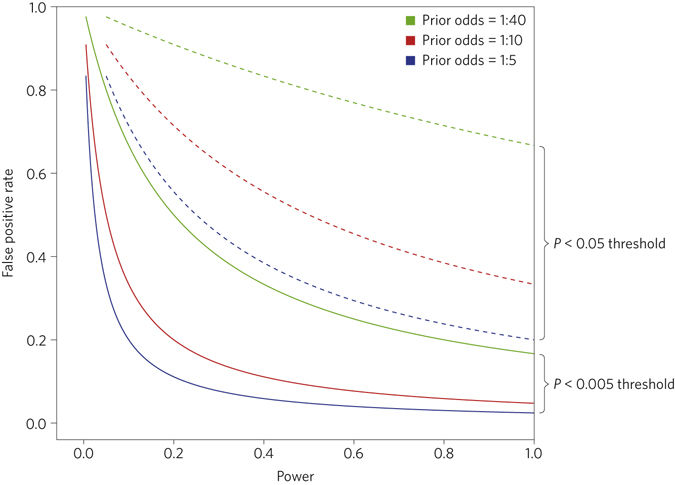
\includegraphics[width=.85\textwidth]{./frequentFigs/power_v_p}
\end{frame}

\section{(July 24) Solution 2: Quantify model likelihood }
\begin{frame}[fragile]
  \frametitle{Briggs}
  Anybody can check [the model likelihood]’s predictions, even if they do not know [the data] or [the model]’s details. Given [the model and the data], authors might claim there is a 55\% chance Y is true under the new protocol. Any reader can verify whether this prediction is useful for him or not, whether the predictions are calibrated, etc.
\end{frame}



\section{Solution 3: Abandon Statistical Significance}
\begin{frame}[fragile]
  \frametitle{McShane}
  \begin{itemize}
  \item Any thresholds will be circumvented by bad practice
  \item Higher thresholds don't mean more true
  \item Higher thresholds breed overconfidence
  \item NHST promote pairwise comparisons instead of total data
  \item Statistical tests do not remove personal bias
  \end{itemize}
\end{frame}

\begin{frame}[fragile]
  \frametitle{McShane}
  Proposal:
  \begin{itemize}
  \item Limit p-values to screening
  \item Include more evidence than just p-values
  \item Judge the research based on all results
  \end{itemize}
\end{frame}


\end{document}
